% Please use the skeleton file you have received in the
% invitation-to-submit email, where your data are already
% filled in. Otherwise please make sure you insert your
% data according to the instructions in PoSauthmanual.pdf
\documentclass{PoS}
\usepackage{lipsum}

%\usepackage{subfigure}
%\usepackage{hepnames}
%\usepackage{hyperref}

%\usepackage[amssymb]{SIunits} %FIXME SIunits or siunitx ?
\usepackage[load-configurations=abbreviations,tight-spacing=true,separate-uncertainty,bracket-numbers = false]{siunitx} 

\usepackage{graphicx}% Include figure files
\usepackage{subfigure}

\usepackage{lineno}
\setpagewiselinenumbers
\modulolinenumbers[5]

%FIXME always copy this list to next telescope paper!
%general stuff 
\newcommand{\e}{\ensuremath{\mathnormal{e}}}
\newcommand{\h}{\ensuremath{\mathnormal{h}}}
\newcommand{\eV}{\ensuremath{\textrm{eV}}}
\newcommand{\cspeed}{\ensuremath{\mathnormal{c}}}
\newcommand{\dd}{\mathrm d}

%tscope specific
\newcommand{\DESY}{\ensuremath{\textrm{DESY}}}
\newcommand{\Datura}{\ensuremath{\textrm{DATURA}}}
\newcommand{\Duranta}{\ensuremath{\textrm{DURANTA}}}
\newcommand{\Mimosa}{\ensuremath{\textrm{MIMOSA\,26}}}
\newcommand{\noise}{\ensuremath{\xi_{\textrm{n}}}}
\newcommand{\epsdut}{\ensuremath{\mathnormal{\varepsilon_{\textrm{DUT}}}}}
\newcommand{\epssut}{\ensuremath{\mathnormal{\varepsilon_{\textrm{SUT}}}}}
\newcommand{\epsmimo}{\ensuremath{\mathnormal{\varepsilon_{\textrm{M26}}}}}
\newcommand{\dz}{\ensuremath{\textrm{d}z}}
\newcommand{\dzsut}{\ensuremath{\textrm{d}z_{\textrm{SUT}}}}
\newcommand{\xzero}{\ensuremath{\mathnormal{X}_0}}

%resolutions
\newcommand{\sigmap}{\ensuremath{\sigma_{\textrm{pointing}}}}
\newcommand{\sigmatu}{\ensuremath{\sigma_{\textrm{t,u}}}}
\newcommand{\sigmatb}{\ensuremath{\sigma_{\textrm{t,b}}}}
\newcommand{\sigmat}{\ensuremath{\sigma_{\textrm{t}}}}
\newcommand{\sigmapGBL}{\ensuremath{\sigma_{\textrm{p,GBL}}}}
\newcommand{\sigmameas}{\ensuremath{\sigma_{\textrm{meas}}}}
\newcommand{\sigmadut}{\ensuremath{\sigma_{\textrm{DUT}}}}
\newcommand{\sigmai}{\ensuremath{\sigma_{\textrm{int}}}}
\newcommand{\sigmam}{\ensuremath{\sigma_{\textrm{M26}}}}
\newcommand{\sigmahat}{\ensuremath{\hat{\sigma}_{\textrm{int}}}}
\newcommand{\sigmaslope}{\ensuremath{\sigma_{\textrm{slope}}}}
\newcommand{\sigmaeps}{\ensuremath{\sigma_{\textrm{eps}}}}
\newcommand{\sigmaedge}{\ensuremath{\sigma_{\textrm{edge}}}}

%positions
\newcommand{\zdut}{\ensuremath{z_{\textrm{DUT}}}}
\newcommand{\zzz}{\ensuremath{z_{3}}}

%residuals
\newcommand{\rbiased}{\ensuremath{r_{\textrm{b}}}}
\newcommand{\runbiased}{\ensuremath{r_{\textrm{u}}}}
\newcommand{\rhat}{\ensuremath{\hat{r}_{\textrm{b}}}}
\newcommand{\pb}{\ensuremath{p_{\textrm{b}}}}

%angles
\newcommand{\aeff}{\ensuremath{\alpha_{\textrm{eff}}}}

%software
\newcommand{\eudet}{\ensuremath{\textrm{EUDET}}}
\newcommand{\eudaq}{\ensuremath{\textrm{EUDAQ}}}
\newcommand{\EUTelescope}{\ensuremath{\textrm{EUTelescope}}}
\newcommand{\Geant}{\ensuremath{\textrm{Geant4}}}

\title{Material budget measurements with beam telescopes}

\ShortTitle{Material budget measurements with beam telescopes}

\author{\speaker{Hendrik Jansen}\\
        DESY\\
        E-mail: \email{hendrik.jansen@desy.de}}

\author{Paul Sch\"utze\\
        DESY\\
        E-mail: \email{paul.schuetze@desy.de}}

\abstract{
High-precision particle tracking devices allow for two-dimensional analyses of the material budget distribution of, e.g., particle detectors and their periphery.
These tracking devices, called beam telescopes, enable a precise measurement of the trajectory of charged particles with an angular resolution in the order of a few ten microradian
 and a position resolution of a few micrometer.
In this contribution, the material budget of a structured aluminum cube is reconstructed from various estimators based on the deflection angles of simulated electron trajectories.
Electrons in the GeV-range serve as beam particles carrying enough momentum to traverse few millimetre thick targets
 whilst undergoing multiple Coulomb scattering in the target allowing for precise measurement of the deflection. 
Probing a target under various rotation angles with respect to the beam axis enables a tomographic reconstruction of the target. 
 
We discuss the performance of the estimators and their impact on the contrast and resolution of the reconstructed image. 
}

\FullConference{The 26th International Workshop on Vertex Detectors\\
		10-15 September, 2017\\
		Las Caldas, Asturias, Spain}


\begin{document}
\linenumbers
\section{Introduction}
%\lipsum
Understanding the scattering of charged particles off nuclei in different materials has been of interest for many decades. 
Moli\`ere~\cite{moliere} postulated a theory without empirical parameters to describe multiple scattering in arbitrary materials.
Later, Gaussian approximations to the involved calculations of his theory have been developed e.g.\ by Highland~\cite{ref:scatteringhighland} in order to simplify predictions.

Today, precise tracking detectors allow for the characterisation of unknown materials based on their scattering properties. %try to avoid single phrase paragraphs, I guess.
In this contribution, measurements with the $\Datura$ beam telescope, a high-precision tracking device consisting of silicon pixel sensors, are described.
The scattering behaviour of GeV electrons traversing aluminium targets with precisely known thicknesses between \SI{13}{\um} and \SI{e4}{\um} at the DESY test beam facility are studied.
A track reconstruction is performed, enabling the extraction of the particle scattering angles at the target arising from the multiple scattering therein.


\section{Simulation set-up}
% Describe setup, sensors and sample
For the simulation presented, the AllPix~\cite{ref:AllPix} detector simulation framework was used. 
Being based on the $\Geant$ libraries~\cite{ref:Geant4}, it includes a realistic model of the interaction of a high-energy particle beam with matter
 and therefore an implementation of multiple Coulomb scattering processes.
Furthermore, the AllPix framework allows for the definition of active sensor volumes,
 emulating the response of particle detectors using a data-driven digitization process. 

The simulation mimics a realistic set-up, as it can be realised at the DESY Test Beam Facility~\cite{ref:DESYtb}. 
Six pixelated  silicon sensor planes, representing the DATURA beam telescope~\cite{JansenEPJ}, are positioned around a sample under test (SUT), cf.\ Fig.~\ref{fig:setup}~(left). 
%The sensor planes resemble six MIMOSA 26 fine-pitch pixel sensors. 
%With a pixel pitch of $\SI{18.4}{\mu}\times \SI{18.4}{\mu}$ and an array of 1152 columns and 576 rows, each sensor covers a total area of $\SI{21.2}{m\meter}\times\SI{10.6}{m\meter}$. 
Each time a simulated particle traverses one of the 
%$\SI{50}{\mu}$ thin 
sensor planes, a response signal is calculated. In this case, these signals are clusters of one or more firing pixels, depending on the impact position of the particle and trimmed to their measured response~\cite{ref:datura-inpixel}.
% The intrinsic sensor resolution has been measured to be $\SI{3.24}{\mu}$.

The simulated SUT, shown in Fig.~\ref{fig:setup} (right), is an aluminium cube with an edge length of $\SI{6}{\mm}$,
 featuring a rectangular cut-out of $\SI{3}{\mm}\times\SI{3}{\mm}\times\SI{1.5}{\mm}$ at the bottom side. 
Furthermore, squared and round holes ranging from $\SI{0.1}{\mm}$ to $\SI{1}{\mm}$ in size and diameter are added.% in order to investigate on the visibility of small structures.

\begin{figure}[!b]
	\center
	\includegraphics[trim= 50 180 220 20, width=.45\linewidth]{figures/sketch_tscope_phantom.eps}
	\hspace{30pt}
	\raisebox{33pt}{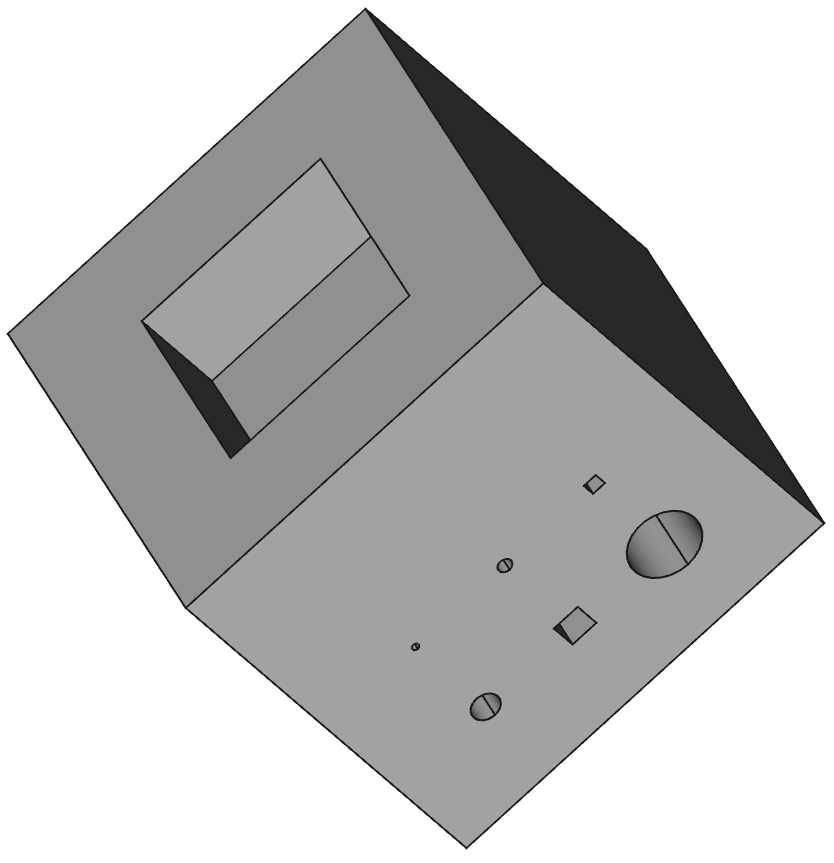
\includegraphics[trim= 0 0 0 0, width=.17\linewidth]{figures/phantomTest.png}}
	\caption[Sketch of the Datura beam telescope]{Sketch of the $\Datura$ beam telescope (left) with its six pixel detector planes and the sample under test (SUT) shown in 3D (right). % with six sensor planes and a sample under test in the centre (left). 
	%The sample, shown in 3D (right), consists of a $\SI{6}{m\meter}$ aluminium cube with a rectangular cut-out as well as round and rectangular holes of different sizes.
	}
	\label{fig:setup}
\end{figure}

In the chosen configuration, the sample is placed in the centre of the beam telescope, half way between plane\,2 and plane\,3, as shown in Fig.~\ref{fig:setup}. %counting (``second'' is ambigious ...)
Whereas the distance $\dzsut$ between the SUT and the neighbouring sensors is minimised in order to yield a good pointing resolution at the sample,
 the distances $\dz$ between two sensor planes are maximised for a more precise angle measurement.
Here, the distances were chosen to be $\dzsut =\SI{10}{\mm}$ and $\dz=\SI{150}{\mm}$. 
An electron beam with a momentum of $\SI{1.6(4)}{\giga\eV/\cspeed}$ and a divergence of $\SI{1}{\milli\radian}$ is used to fully illuminate the sample. 

The $\Geant$ libraries include a physics model emulating, among other things, energy losses due to ionization and scattering processes.
Charged particles traversing any material are deflected by the electric field of the nuclei, resulting in an effective deflection of the particle in the transverse plane,
 which depends on the material budget $\varepsilon$ traversed. 
As an approximation to the Moliere theory, the distribution of scattering angles follows a normal distribution with the variance given by~\cite{ref:scatteringhighland, ref:pdg2016} 

\begin{equation}
 \Theta_0^2 = \left( \frac{\SI{13.6}{\mega\eV}}{\beta \cspeed p}\cdot z \right)^2 \cdot \varepsilon \cdot \big( 1+0.038\cdot\ln(\varepsilon) \big)^2\,,
 \label{eq:highland}
\end{equation}

\noindent
with the particle's velocity $\beta \cspeed$, its momentum $p$ and its charge number $z$. 
Hence the material budget and therefore the material properties of a sample can be extracted from a measurement of the scattering angle distribution.

In order to account for an inhomogeneous response of the measurement system,
 the measurement of such distributions for homogeneous samples of known material type and thickness can be used to calibrate the measured response, as implied in~\cite{ref:X0}.

\section{Material budget estimators}

criteria:

- robust (dependence on population)
- accurate (similar to HL)
- unbiased (no boundaries while filling)

- Gaussian width of linearly filled
- RMS of linearly filled 
- Student t of linearly filled

- sqrt of mean of quadratically filled



\section{Results}
\paragraph{Contrast}

- GBL vs triplet in 2D (based on constrast)

\paragraph{Resolution vs contrast}

- reso vs contrast for various bin sizes


\section{Conclusion}




\begin{thebibliography}{99}
\bibitem{...}
....

\end{thebibliography}

\end{document}
